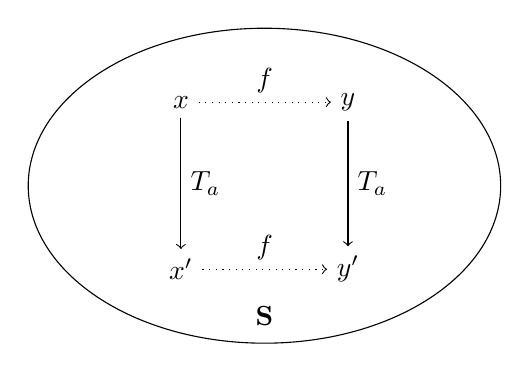
\begin{tikzpicture}
\usetikzlibrary{calc}

% Draw state spaces as rectangles
\draw (0,0) ellipse (3 and 2);
% Draw state space labels
\node at (0,-1.65) {$\mathbf{S}$};

% Xs
\node (x1) at ($(0,0) - (-45:1.5)$) {$x$};
\node (x2) at ($(0,0) - (45:1.5)$) {$x'$};
\draw[->] (x1) to node[auto]{$T_a$}  (x2);

% Ys
\node (y1) at ($(0,0) + (45:1.5)$) {$y$};
\node (y2) at ($(0,0) + (-45:1.5)$) {$y'$};
\draw[->] (y1) to node[auto]{$T_a$}  (y2);

% Map
\draw[->,dotted] (x1) to node[auto]{$f$} (y1);
\draw[->,dotted] (x2) to node[auto]{$f$} (y2);

\end{tikzpicture}